\begin{wrapfigure}[12]{r}[0pt]{55mm}
	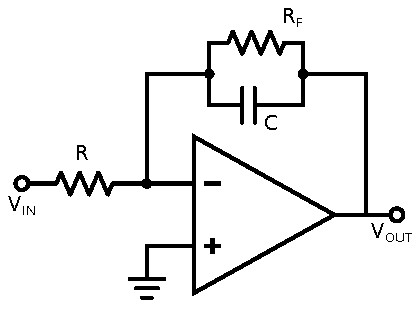
\includegraphics[width=55mm]{ccint.pdf}
	\caption{Circuito integratore}
	\label{fig:ccint}
\end{wrapfigure}

\section{Integratore}

In questa parte dell'esperienza utilizzeremo un op-amp per costruire un circuito integratore. Analizzando lo schema riportato in Fig. \ref{fig:ccint}, assumendo che $R_f=\infty$\footnote{Senza tale approssimazione risulta particolarmente complicata la trattazione del circuito.}, è semplice ricavare $I=C\frac{d(V_A-V_{out})}{dt}$ da cui $V_{in}=-RC\frac{V_{out}}{dt}$.

Vale la seguente relazione:%Non siamo matematici ma la seguente relazione è triviale:

\begin{equation}
V_{out}=-\frac{1}{RC} \int V_{in}dt +costante
\label{eq:int}
\end{equation}

I valori di resistenze e capacità utilizzate sono $R=(99.2 \pm 0.1)$ \si{\kilo\ohm},\\
$R_f=(2.247 \pm 0.001)$ \si{\mega\ohm} e $C=(0.097 \pm 0.002)$ \si{\micro\farad}. 

Poiché nel circuito è presente un condensatore, dobbiamo preoccuparci di calcolare la frequenza di taglio.
Considerando la presenza di un'op-amp e la struttura del circuito, esso funzionerà meglio a frequenze basse che a frequenze alte (un condensatore a basse frequenze si comporta come un circuito aperto, ad alte frequenze come un filo ideale).
Assumendo trascurabili i contributi dati da $R_f$ e dalla resistenza interna dell'oscilloscopio (la prima molto grande, dell'ordine del $\si{\mega\ohm}$, la seconda messa in parallelo con l'impendenza in uscita del'op-amp\footnote{Ricordiamo che l'impedenza in uscita dell'op-amp è praticamente nulla in quanto abbiamo un transistor fet che porta direttamente a ground.}), la frequenza di taglio è stimabile da $f\simeq \frac{1}{2\pi C R_1}$.
Inserendo i valori numerici otteniamo $f \simeq \SI{15}{\hertz}$.
Il circuito si comporterà all'incirca come un filtro passa basso.
Abbiamo dunque deciso di utilizzare dei segnali in ingresso a frequenza di \SI{10}{\hertz}.
Abbiamo tuttavia provato anche per frequenze di \SI{1}{\kilo\hertz}.
I risultati sono esposti nei seguenti grafici.

$$Grafici$$

Come vediamo, anche per alte frequenze rispetto a quella di taglio (100 volte) il circuito funziona ancora come integratore. 
%sebbene ci sia un fattore moltiplicativo inferiore a 1 che modula l'integrale.
Inoltre si noti la presenza di un offset sovrapposto al segnale in uscita. Tale tensione continua è la costante di Eq. \eqref{eq:int}



Abbiamo successivamente provato a togliere la resistenza di feedback $R_f$.
Dalla teoria sappiamo che tale circuito in linea ideale è instabile per frequenze troppo basse, in quanto non abbiamo un circuito di retroazione e dunque non riusciamo a controllare il segnale in output.
In pratica, poichè l'op-amp non è ideale, il circuito non funziona mai.
Infatti, per frequenze alte abbiamo visto in uscita un segnale che cresceva nel tempo.
Pensiamo che il motivo che spiega tale fenomeno sia la non perfetta simmetria dell'amplificatore operazionale.
Se così fosse infatti, avremmo che il condensatore tende a caricari positivamente in quanto il valore di tensione di clapping positivo era, in modulo, maggiore di quello negativo.
